% Name: Plot from an inline table
% Description: Reaction, braking, and total stopping distance against speed, all read from one table written in the source, the total computed from two of its columns.
% Tags: table, data, stopping distance, line plot

\usepackage{pgfplots}
\usepackage{pgfplotstable}
\pgfplotsset{compat=1.18}

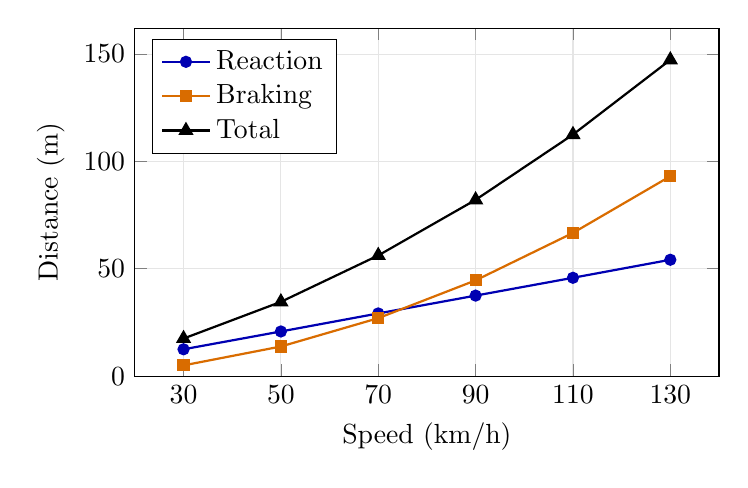
\begin{tikzpicture}
  % Reaction distance for a 1.5 s reaction time; braking distance v^2/(2a) at a = 7 m/s^2.
  \pgfplotstableread{
    speed  reaction  braking
    30     12.5      5.0
    50     20.8      13.8
    70     29.2      27.0
    90     37.5      44.6
    110    45.8      66.7
    130    54.2      93.1
  }\stopping
  \begin{axis}[
    width=9cm, height=6cm, xlabel={Speed (km/h)}, ylabel={Distance (m)},
    xtick={30,50,...,130}, ymin=0, legend pos=north west, legend cell align=left,
    grid=major, grid style={gray!20}, every axis plot/.append style={thick, mark size=1.8pt},
  ]
    \addplot[blue!70!black, mark=*] table[x=speed, y=reaction] {\stopping};
    \addplot[orange!85!black, mark=square*] table[x=speed, y=braking] {\stopping};
    \addplot[black, mark=triangle*, mark size=2.4pt] table[x=speed, y expr=\thisrow{reaction} + \thisrow{braking}] {\stopping};
    \legend{Reaction, Braking, Total}
  \end{axis}
\end{tikzpicture}
